\section{Aerostructure} %Liana
\label{sec:aerostructure}
The airframe consists of three main parts: the nosecone, the body tube and the fincan. These are connected by aluminium coupler rings, whereby the one that connects the nosecone and body tube is described in detail in the recovery section (\cref{sec:recovery}). Most of the parts are made in-house, so besides the idea behind the design, the process of manufacturing is outlined.

\subsection{Nosecone}
Based on the Von Kármán shape, the nosecone (shown in \Cref{fig:aerostructure_nosecone}) optimizes the airflow around the rocket and minimizes drag. Due to being made of glass fiber, it is transparent to electromagnetic radiation, making it the RF window of the rocket.

The glass fiber mats were wet laminated to a positive 3D-printed mold with epoxy resin in three layers. The surface was then sanded and touched up evenly in several passes before the 3d-printed core was removed.
This \SI{360}{\milli\meter} long center part is enclosed by the \SI{42.25}{\milli\meter} lathed aluminum tip that is screwed into a mounting piece at the top and a aluminium coupler ring serving as a recovery separation mechanism connecting it to the body tube at the bottom, which is described in more detail at \cref{sec:recovery}.

\begin{figure} [H]
\centering
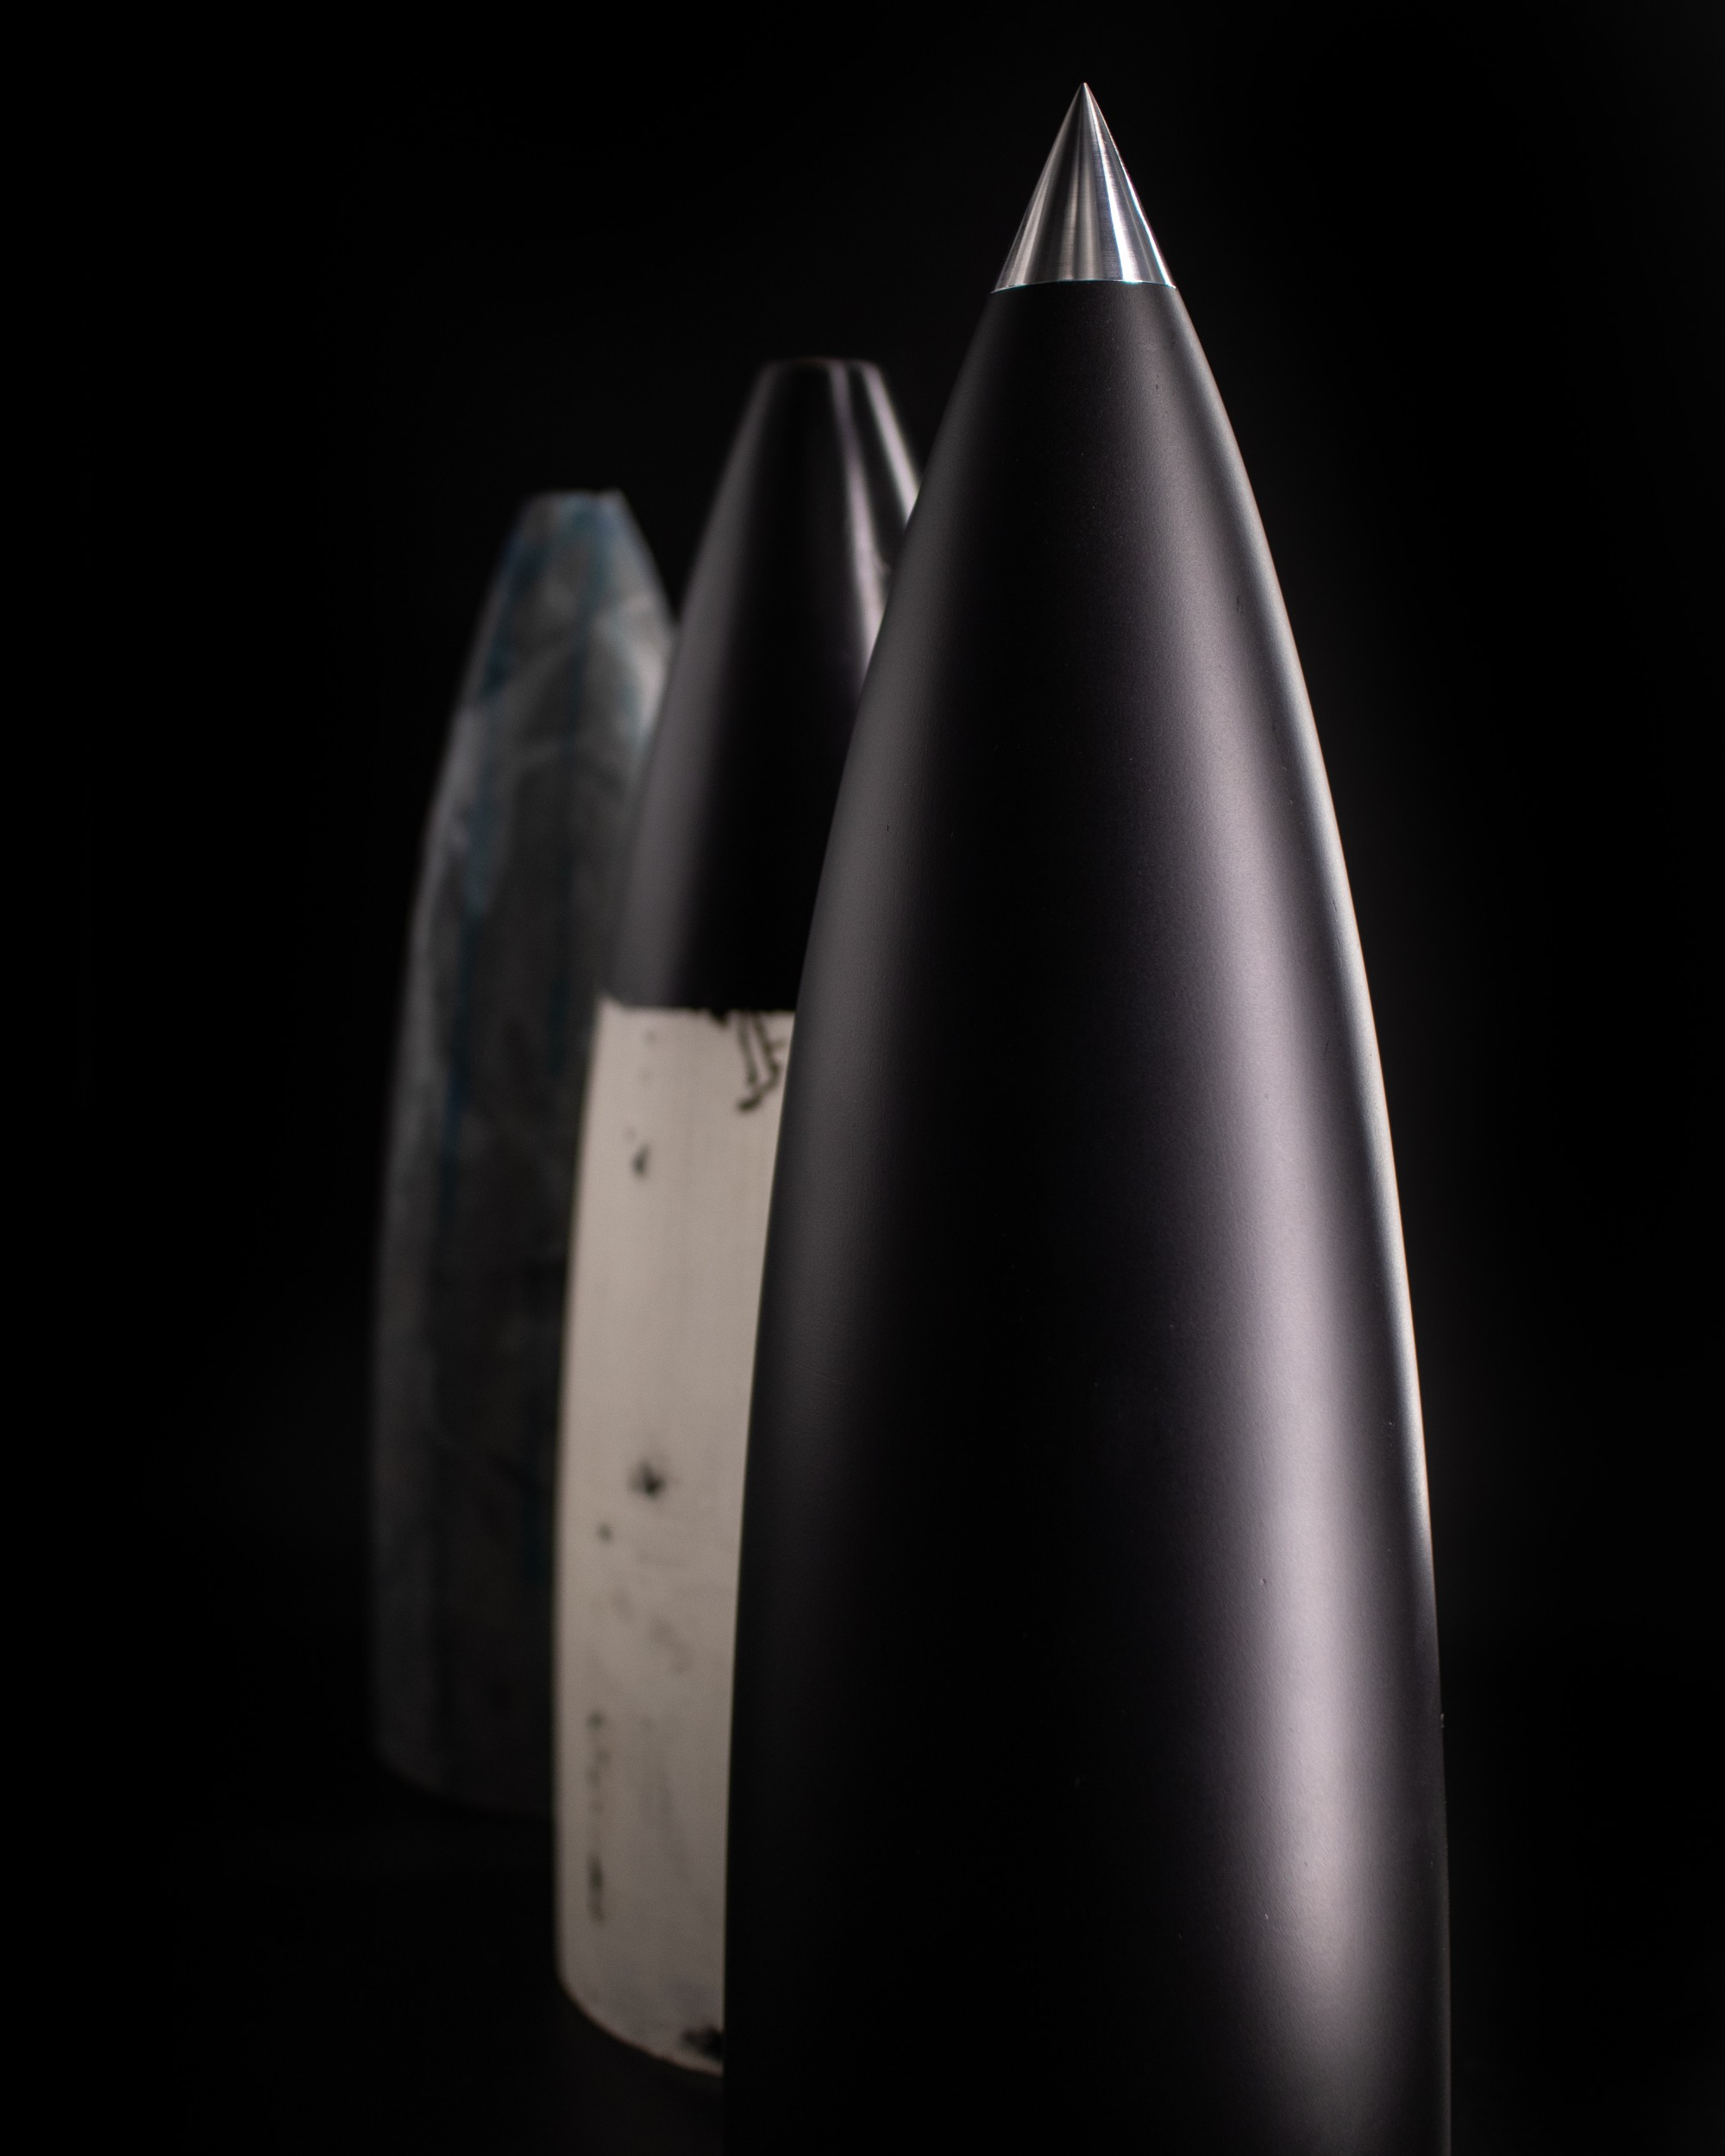
\includegraphics[width=0.5\textwidth]{Aerostructure/NC_4 (2).jpg}
\caption{Different versions of the nosecone, improvements from back to front (final version). The black paint was removed after a test flight and replaced with a white coat.}
\label{fig:aerostructure_nosecone}
\end{figure}

\subsection{Body Tube}
The body tube has an outer diameter of \SI{123}{\milli\meter} and a wall thickness of \SI{1.5}{\milli\meter}. It consists of radially wound carbon fiber inner layers and weaved outer layers and was manufactured to spec externally.

\subsubsection{Umbilical Feedthroughs}
To make fueling, arming and setting up pad-communication convenient, easily accessible connectors and mechanisms are necessary while the rocket is on the launchpad. For this purpose, openings for the connections are provided on the side of the airframe.

\subsubsection{Launch Pad Mechanical Interface}
The vehicle is connected to the launch rail using two rail buttons made of brass. The location of the upper rail button influences both the stability on the rail as well as the effective length of rail available for stabilization during launch. It is mounted with the screw that is also used to hold the fuel tank. The bottom rail button is used to support the weight of the vehicle while on the launch pad and to hold it down until successful engine ignition is confirmed. It is screwed to the airframe fincan coupler.

\subsubsection{Airframe-Fincan Coupler}\label{sec:aerostructure_lowercoupler}
Fincan and body tube are joined using an aluminium coupler ring that provides a tight fit and is held in place via radial screws. This ring is also where the thrust from the engine is introduced into the airframe, using four aluminium struts that connect the coupler ring to the engine head. This is explained in more detail under \Cref{sec:engine_valves_fill_connections}.

\subsection{Fincan}
To bring the center of pressure well below the center of gravity and thus ensure sufficient static stability, we opted for four fins and a lightweight carbon fiber construction. The fillets between fins and center piece are designed rather extensive, so that those areas are resistant enough.

The Fin profile is based on a symmetrical airfoil profile and was then adapted so that a positive mold could be 3D-printed in house. This mold was sanded and treated with several thin layers of coat to seal pores and after that with release agent. Then a four-part negative mold consisting of high-temperature epoxy tooling gelcoat and high-temperature epoxy moulding paste was taken. This was then used to laminate with pre-preg carbon fiber. For the fin cores Rohacell, a closed-cell rigid foam, was chosen. Those inlays are both essential for the stiffness of the fins and ensure that enough pressure is exerted on the laminate during the curing process. The Boards of Rohacell foam were CNC-milled to the correct form and then placed on the four layers of carbon fiber mats before the negative mold was assembled. The inside of the tincan was strengthened with another two layers of carbon fiber. After being sealed in a vacuum bag and cured by by being gradually heated to 135°C in the oven, the fincan was sanded, cut down to the lengh of \SI{300}{\milli\meter} and prepared for painting (shown in \Cref{fig:aerostructure_fincan})

\begin{figure} [H]
\centering
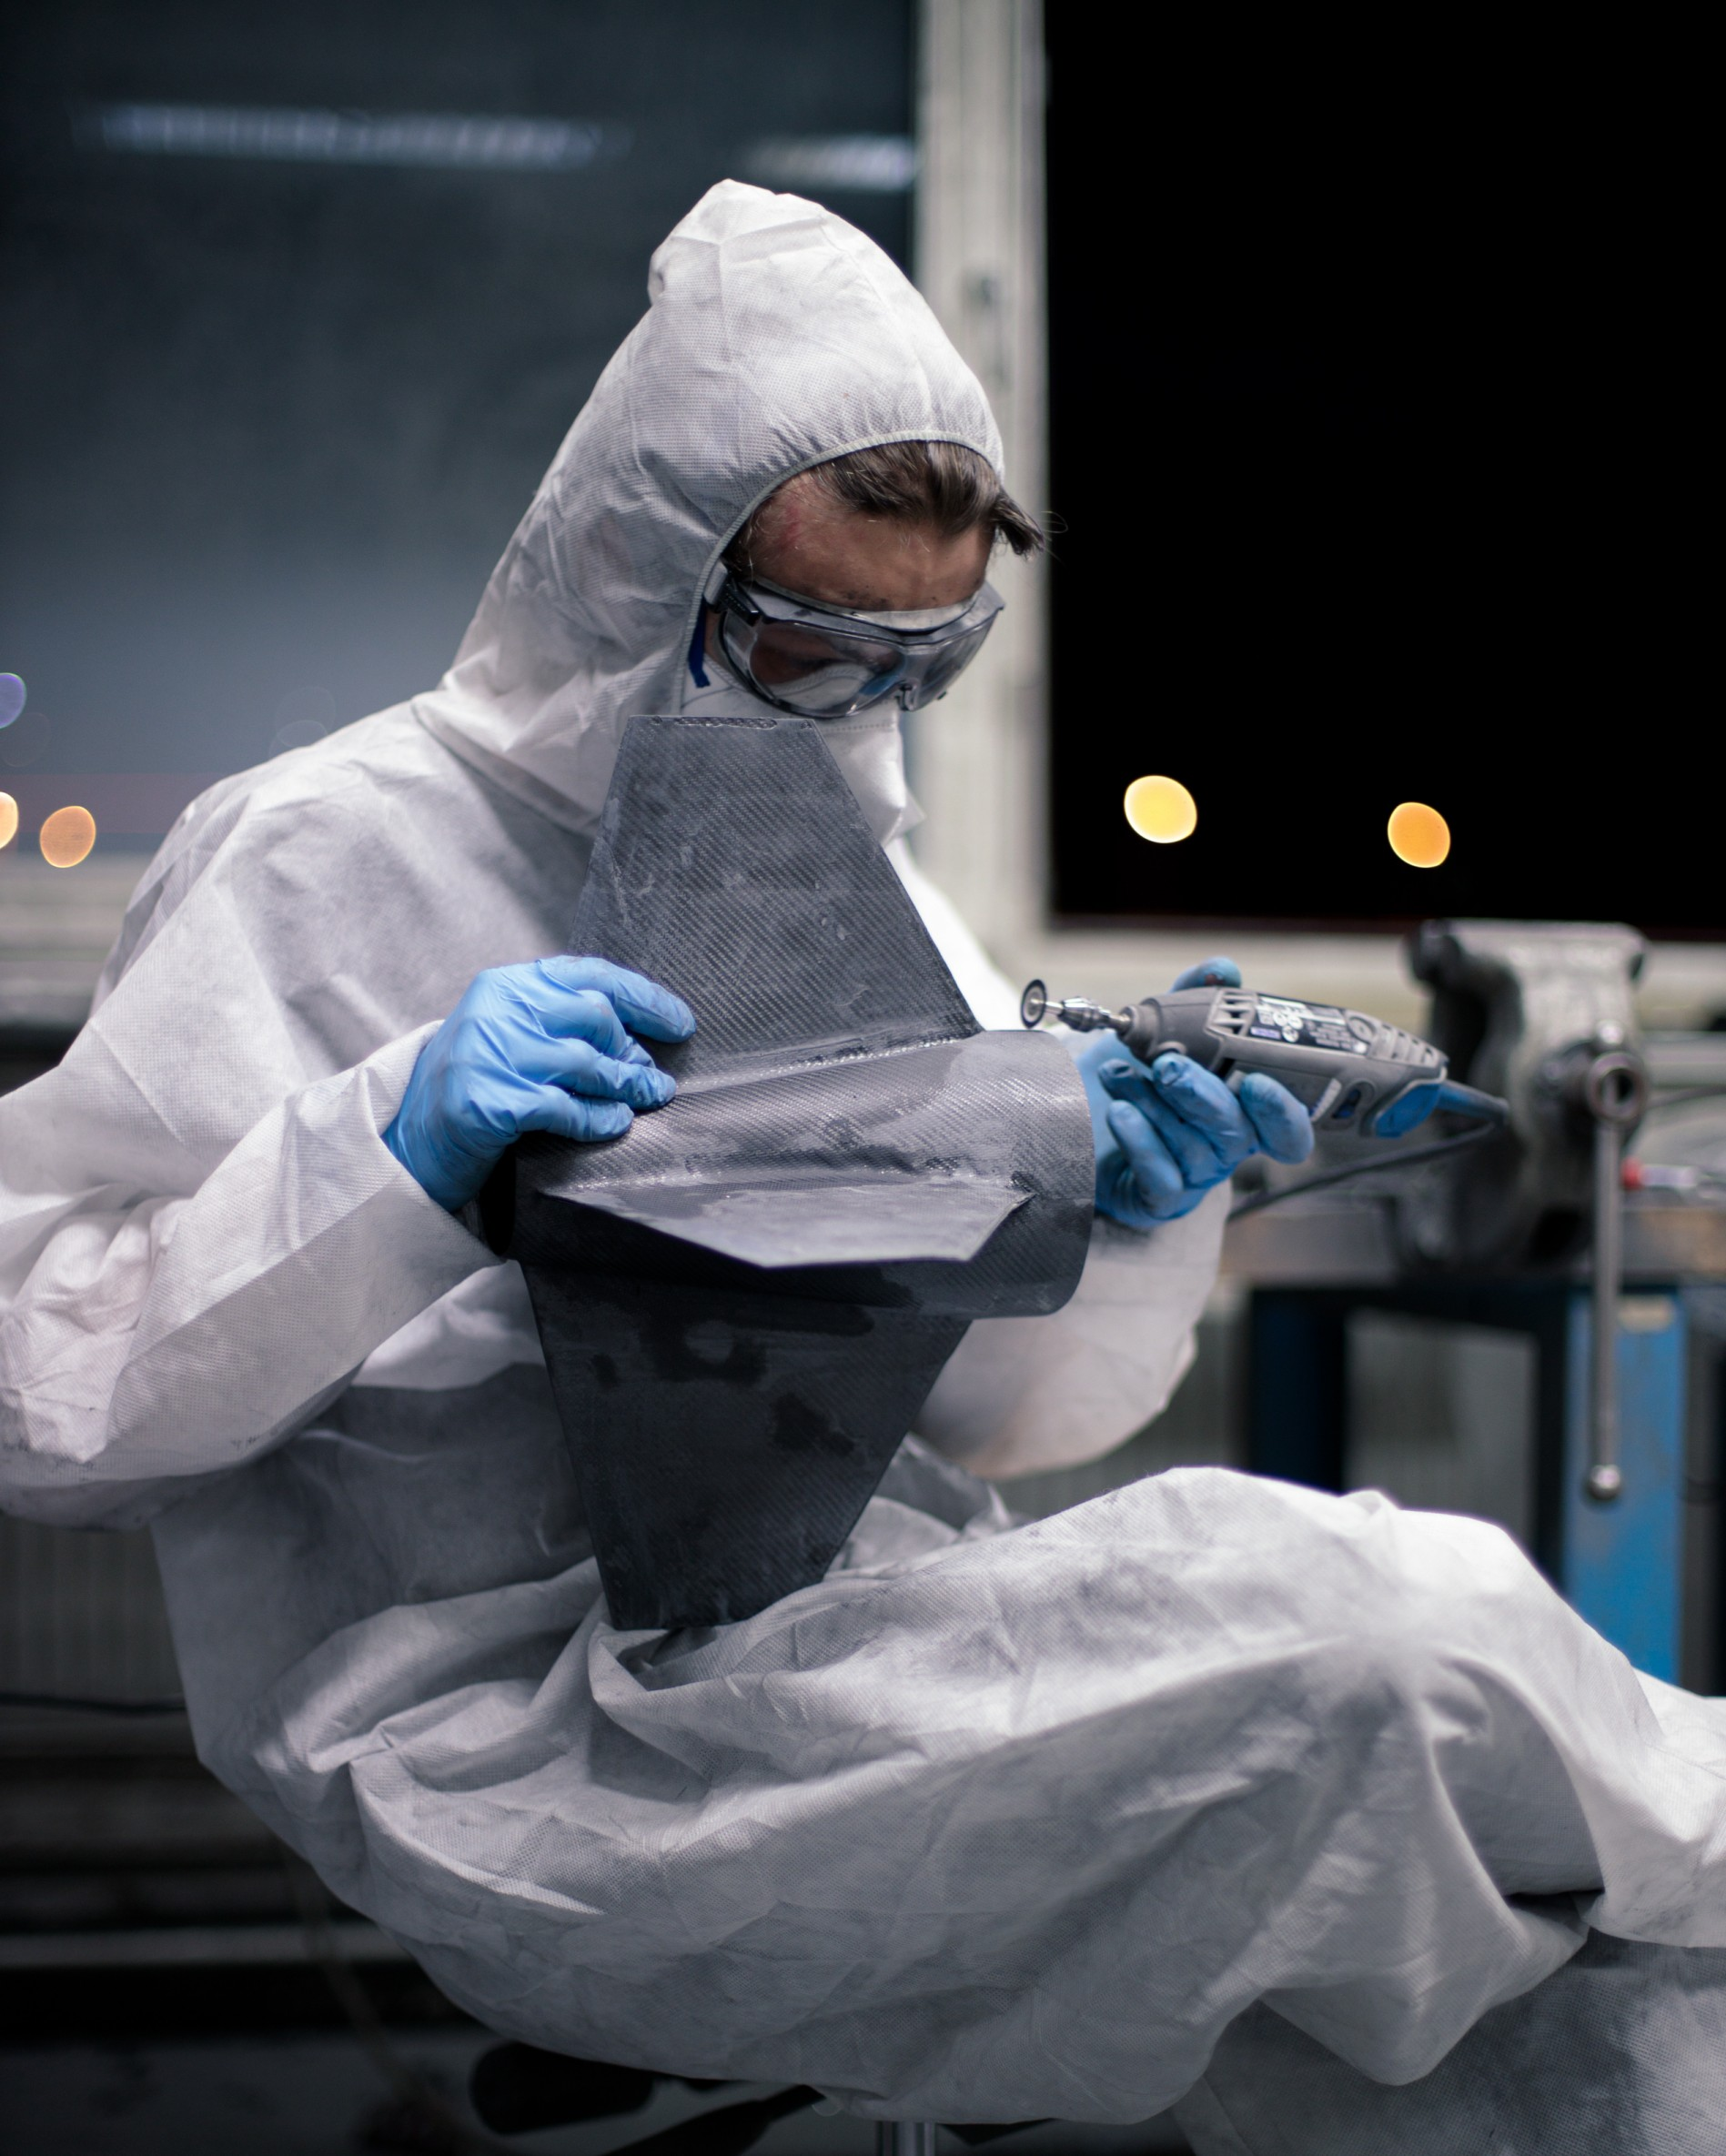
\includegraphics[width=0.5\textwidth]{Aerostructure/Fincan-3.jpg}
\caption{Surface sanding after curing of the Fincan.}
\label{fig:aerostructure_fincan}
\end{figure}

\subsection{Livery Design and Surface Finish}
To accomplish a flawless look as well as create a surface that mitigates some of the solar heating experienced in the EuRoC launch environment, the airframe is painted white. The decision was made in favor of lacquer and against adhesive foil, since the latter has proven to be both unsightly and less resistant. Furthermore, painting allows to not have solid black markings, but to leave the carbon fiber underneath visible, which displays the lamination work and the texture of the airframe.

On the body tube the team name, the project name, the academic affiliation and the sponsor logos are arranged into a minimalistic design. The fins all feature the Team ID and the Austrian flag. Each of them additionally displays a unique but simple graphic pattern of black and white to allow ground-based observers to track and record the launch vehicle’s altitude.

To achieve a satisfactory result, first the flaws were repaired with epoxy resin, then the whole airframe was sanded and coated with transparent primer. After drying, stencil stickers were applied in the places of the markings. The white paint was then sprayed on and allowed to harden. The stickers were then carefully removed and the airframe covered with a clear, matte two-component coat.